\documentclass[10pt]{article}
\usepackage[margin=0.75in]{geometry}
\usepackage{makecell}
\usepackage{longtable}
\usepackage{amsmath, amssymb}
\usepackage{listings}
\usepackage{xcolor}
\usepackage{tikz}
\usepackage{tcolorbox}
\tcbuselibrary{skins, breakable}

\lstdefinestyle{bashconsole}{
    backgroundcolor=\color{black!5},
    basicstyle=\ttfamily\color{black},
    keywordstyle=\color{blue}\bfseries,
    commentstyle=\color{green!70!black},
    stringstyle=\color{red!70!black},
    numberstyle=\tiny\color{gray},
    breaklines=true,
    frame=single,
    rulecolor=\color{black!20},
    xleftmargin=0.5cm,
    numbers=left,
    numbersep=5pt,
    literate={\$}{{\textcolor{blue}{\$}}}1,
    showstringspaces=false,
    upquote=true,
}

\usetikzlibrary{shapes.geometric, arrows}

\tikzstyle{startstop} = [rectangle, rounded corners, minimum width=3cm, minimum height=1cm,text centered, draw=black, fill=red!30]
\tikzstyle{process} = [rectangle, minimum width=3cm, minimum height=1cm, text centered, draw=black, fill=orange!30]
\tikzstyle{decision} = [diamond, aspect=2, text centered, draw=black, fill=green!30]
\tikzstyle{arrow} = [thick,->,>=stealth]

\definecolor{mauve}{rgb}{0.58,0,0.82}

\lstdefinelanguage{assembly}{
  alsoletter={.}, % allow dots in keywords
  alsodigit={0x}, % hex numbers are numbers too!
  morekeywords=[1]{ % instructions
    load, loadu, loadi, zero, store,
    add, sub, mul, div, mod,
    cmp, jmp, jal, b, beq, bne, bge, bgt, ble, blt, bz, bnz,
    not, and, xor, or, shr, shl,
    syscall, nop, exit, int, rti
  },
  morekeywords=[2]{
    define, end, include, macro, rm, stop
  },
  morekeywords=[3]{
    \$ip, \$rip, \$sp, \$fp, \$flag, \$isr, \$imr, \$iip, \$ret,
    \$k1, \$k2,
    \$r1, \$r2, \$r3, \$r4, \$r5, \$r6, \$r7, \$r8, \$r9, \$r10, \$r11, \$r12, \$r13, \$r14, \$r15, \$r16, \$r17, \$r18, \$rt19, \$r20, \$r21
  },
  commentstyle=,
  morecomment=[l]{;},   % mark ; as line comment start
  morestring=[b]",      % mark " as string start/end
  morestring=[b]'       % also mark ' as string start/end
  % listings sonderzeichen (for german weirdness)
}

\lstdefinestyle{assembly}{
  language=assembly,
  basicstyle=\ttfamily,
  breaklines=true,
  commentstyle=\itshape\color{green!50!black},
  keywordstyle=[1]\color{blue!80!black},
  keywordstyle=[2]\color{orange!80!black},
  keywordstyle=[3]\color{red!50!black},
  stringstyle=\color{mauve},
  identifierstyle=\color{teal},
  frame=l,
  tabsize=2,
  showstringspaces=false
}

\setlength{\parindent}{0pt}

\title{Assembler Documentation}
\author{Ruben Saunders}
\date{August 2024}

\begin{document}

\maketitle
\tableofcontents

\newpage

\section{Overview}

The assembler takes \textbf{one} assembly source file and produces a binary output file, which may be executed by the processor.

\textbf{Disclaimer}: The assembly language designed for this project is relatively simplistic.
Its goal is to allow for full operation of the processor with minimal-to-no additional features.
This is so focus can be given to the development of a high-level language.

\subsection{Command-Line Interface}

The assembler executable is called as follows:

\medskip
\begin{lstlisting}[style=bashconsole]
$ ./assembler <input_file> -o <output_file> [flags]
\end{lstlisting}

The output file is provided after the \texttt{-o} flag.
The following optional flags are available:
\begin{itemize}
    \item \texttt{-d}: enables debug mode.
    In this mode, detailed results from each step are output to \texttt{stdout}.
    \item \texttt{-l <path>}: path of the library directory (see \texttt{\%include}).
    The library path is calculated by \texttt{<executable path>/<lib path>}, with a default \texttt{<lib path>=url}.
    \item \texttt{--no-pre-process}: skips the pre-processing step.
    \item \texttt{--no-compile}: skips the compilation step.
    \textbf{Note} in this case, the \texttt{-o} flag is not compulsory.
    \item \texttt{-p <filename>}: writes the post-processed source to \texttt{filename}.
    \item \texttt{-r <filename>}: reconstruct the assembly from the compiled output and write it to \texttt{filename}.
\end{itemize}

\subsection{Process Flow}

\bigskip
\begin{tcolorbox}[enhanced, breakable, parbox=false, colback=white]
    \begin{center}
    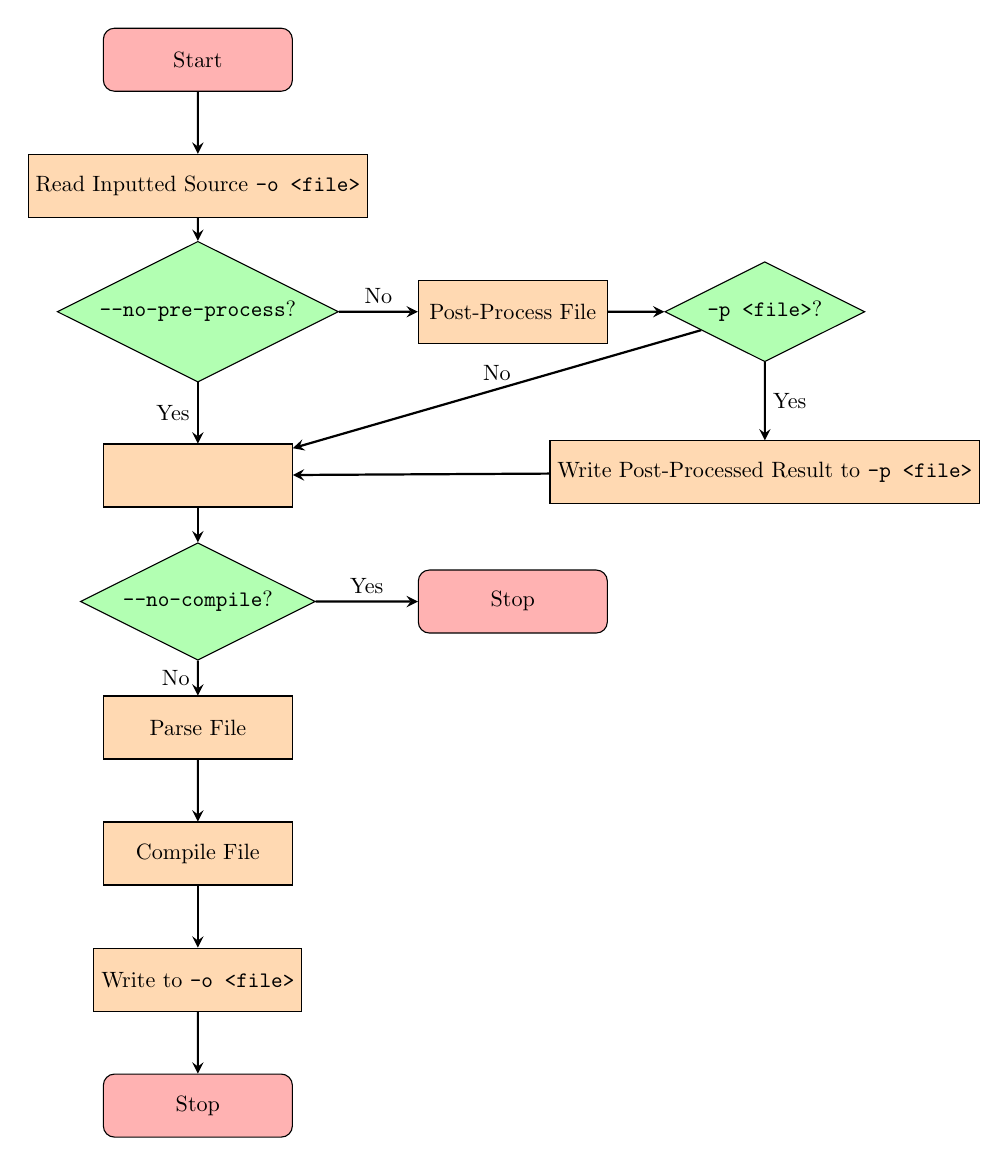
\begin{tikzpicture}[node distance=2cm, scale=0.8, transform shape]
        \node (start) [startstop] {Start};
        \node (process1) [process, below of=start] {Read Inputted Source \texttt{-o <file>}};
        \node (decision1) [decision, below of=process1] {\texttt{--no-pre-process}?};

        \node (process2) [process, right of=decision1, xshift=3cm] {Post-Process File};
        \node (decision2) [decision, right of=process2, xshift=2cm] {\texttt{-p <file>}?};
        \node (process3) [process, below of=decision2, yshift=-0.55cm] {Write Post-Processed Result to \texttt{-p <file>}};

        \node (process4) [process, below of=decision1, yshift=-0.6cm] {};
        \node (decision3) [decision, below of=process4] {\texttt{--no-compile}?};

        \node (stop1) [startstop, right of=decision3, xshift=3cm] {Stop};

        \node (process5) [process, below of=decision3] {Parse File};
        \node (process6) [process, below of=process5] {Compile File};
        \node (process7) [process, below of=process6] {Write to \texttt{-o <file>}};
        \node (stop2) [startstop, below of=process7] {Stop};
    
        \draw [arrow] (start) -- (process1);
        \draw [arrow] (process1) -- (decision1);
        \draw [arrow] (decision1) -- node[anchor=south] {No} (process2);
        \draw [arrow] (decision1) -- node[anchor=east] {Yes} (process4);
        \draw [arrow] (process2) -- (decision2);
        \draw [arrow] (decision2) -- node[anchor=west] {Yes} (process3);
        \draw [arrow] (decision2) -- node[anchor=south] {No} (process4);
         \draw [arrow] (process3) -- (process4);
         \draw [arrow] (process4) -- (decision3);
         \draw [arrow] (decision3) -- node[anchor=south] {Yes} (stop1);
         \draw [arrow] (decision3) -- node[anchor=east] {No} (process5);
         \draw [arrow] (process5) -- (process6);
         \draw [arrow] (process6) -- (process7);
         \draw [arrow] (process7) -- (stop2);
    \end{tikzpicture}
    \end{center}
\end{tcolorbox}

\section{Pre-Processor}

The pre-processor runs prior to compilation.
It modifies the source file's contents before being passed to the compiler.

Core to the pre-processor are \textit{directives}, which are commands to the pre-processor.
Directives are prefixed with a percent (\%) symbol.

\medskip
\begin{longtable}{|c|l|l|}
    \hline
    \textbf{Directive} & \textbf{Signature} & \textbf{Description} \\
    \hline
    Constant Definition & \texttt{\%define <name> <value>} & \makecell[l]{(Re-)Defines a constant \texttt{name} with the given value.\\%
    \textbf{Note} \texttt{<value>} extends to the end of the line.\\%
    \textbf{Note} the start is trimmed of whitespace, but trailing\\%
    whitespace is preserved.} \\
    \hline
    End & \texttt{\%end} & Marks the end of a macro definition. \\
    \hline
    Include File & \texttt{\%include [lib:]<path>} & \makecell[l]{Reads the file contents of \texttt{<path>.asm} and inserts into source.\\%
    \textbf{Note} the \texttt{lib:} prefix navigates to the library directory (specified by the \texttt{-l} flag).} \\
    \hline
    Macro Definition & \texttt{\%macro <name> [<args ...>]} & \makecell[l]{(Re-)Defines a macro with the given name and arguments.\\%
    See the below section for more information.} \\
    \hline
    Ignore Line & \texttt{\%rm <data ...>} & This removes the line from the source. \\
    \hline
    Halt \& Cut & \texttt{\%stop} & \makecell[l]{Stops the pre-processor at this line.\\%
    This and all lines succeeding it are removed from the source.} \\
    \hline
\end{longtable}

\subsection{Macros}

Macros are like pre-processor functions, and may be used to for meta-programming purposes and simplifying code.
Macros have a name and a number of arguments.
The macro's body extends from after the newline to the next \texttt{\%end} directive.
Note that arguments do not have types, as types do not exist at this level.

When referenced, the data after the macro name are split by whitespace and passed position-wise to the arguments.
The argument names are substituted with their values in the macro's body before the reference is itself substituted by this body.

For example,

\begin{lstlisting}[style=assembly]
%macro inc reg
    add reg, reg, 1
%end

inc $r1
\end{lstlisting}

is replaced with

\begin{lstlisting}[style=assembly]
add $r1, $r1, 1
\end{lstlisting}

\section{Assembly Syntax}

After pre-processing is the parsing \& compilation stage.
This section will cover the syntax of the assembly language.
Note that some syntax, such as addressing modes, is covered in the processor documentation document.

The parser reads the source line-by-line, top-to-bottom.
The most common syntax is:

\begin{lstlisting}[style=assembly]
[label:] <mnemonic>[conditional][.datatype] [args ...] [; comment]
\end{lstlisting}

Alternatively, the line may start with a directive.
Note, this is different from a pre-processor directive; see below for more information.

\subsection{Labels}

Labels are defined at start of a line, starting with an alphabetic character or an underscore and any number of alphanumeric characters or underscores, and finally a colon.

A label is a symbol name tied to a memory address; when defined, a label adopts the value of the byte offset in memory.
A label may be redefined, in which case its address value will be updated.

A label is referenced in an argument by stating its name.
How a reference is handles depends on if the label is defined:
\begin{itemize}
    \item If it has been defined, the label is directly substituted by its address as an immediate, \texttt{<imm>}, or as an address reference, \texttt{<addr>}, as expected by the instruction signature.
    \item Otherwise, this is known as a forward-reference.
    This reference is noted and, when the label is defined in the future, this reference will be replaced by the address.
    All forward-references must be resolved by the end of compilation, or an error will be raised.
\end{itemize}

\paragraph*{Special Labels}
There exist a few special labels:
\begin{itemize}
    \item \texttt{main} -- sets the entry point of the program.
    By default, the entry point is \texttt{+0x00}.
    \item \texttt{interrupt\_handler} -- sets the location of the interrupt handler.
    By default, the location of the interrupt handler is \texttt{+0x400}.
\end{itemize}

Special labels may only be declared once.

\subsection{Mnemonics}

Mnemonics are used to introduce instructions, and define the desired function to be taken.
Any arguments supplied provide necessary data for the function to carry out its operation.
The processor documentation document details all legal instructions.

The mnemonic itself consists of three parts.
\begin{itemize}
    \item The base: this is the operation listed in the ISA table, and is the function name.
    \item Conditional test: this is a string such as ``z'', ``eq``, etc. that may be optionally suffixed to most instructions.
    \item Datatype: declared as a suffixed dot followed by a type string, this determines the type of data to be operated on in the case of some instructions.
\end{itemize}

Again, the above table only lists brief description; see the ISA table for more information on each part.

\subsubsection{Pseudo-Instructions}

Pseudo-instructions are marked as such in the processor specification.
As a RISC processor, the instruction set is limited and compact.
Pseudo-instructions are compromises for common operations, written as an intrinsic instruction but expanded into its equivalent intrinsic form by the assembler.

\subsection{Arguments}

The argument types are detailed in the process documentation document, but syntax will be detailed here.
\begin{itemize}
    \item Immediate: a numeric value, e.g., \texttt{42}.
    \item Memory Address: a parenthesised numeric value, e.g., \texttt{(42)}.
    \item Register: a register name suffixed by a dollar `\$', e.g., \texttt{\$r1}.
    \item Register Indirect: a parenthesised register, optionally prefixed by a numeric value, e.g., \texttt{2(\$sp))}.
\end{itemize}

The following list the possible forms of a numeric literal.

\begin{itemize}
    \item Integer: a sequence of digits of a given base.
    A base can be specified with a 0\(b\) prefix, where \(b\) is a base specifier, one of:
    \begin{itemize}
        \item \texttt{b}: binary, base-2.
        \item \texttt{d}: decimal, base-10, the default.
        \item \texttt{o}: octal, base-8.
        \item \texttt{t}: trinary, base-3.
        \item \texttt{x}: hexadecimal, base-16.
    \end{itemize}
    E.g., \texttt{42}, \texttt{0xf5}.
    \item Decimal integer: same as above, but contains a decimal point.
    Bytes are inserted as either a float (32-bit) or double (64-bit).
    E.g., \texttt{3.14}, \texttt{0xf2.e}.
    \item Character literal: a character enclosed in apostrophes yields the character's ASCII value.
    Escape sequences are also supported by using a backslash prefix.
    E.g., \texttt{`a'}, \texttt{`\symbol{92}0'}, \texttt{`\symbol{92}n'}.
\end{itemize}

\subsection{Directives}

Similar to pre-processor directives, these give commands to the compiler and do not relate to actual instructions.
A directive is prefixed with a dot, and must be at the start of a line.

\begin{longtable}{|c|l|l|}
    \hline
    \textbf{Directive} & \textbf{Syntax} & \textbf{Description} \\
    \hline
    \multicolumn{3}{|c|}{\makecell[c]{\textbf{Loading Data}\\%
    These directives are for inserting data into memory in-place.\\%
    Arguments have the same syntax as an \texttt{<imm>}, but may also be strings.\\%
    Strings automatically insert a null character after it is closed.}} \\
    \hline
    Load Byte(s) & \texttt{.byte ...} & Load a sequence of 8-bit bytes into memory.  \\
    \hline
    Load Data & \texttt{.data ...} & Load a sequence of half-words (32-bit) into memory. \\
    \hline
    Load Word(s) & \texttt{.word ...} & Load a sequence of words (64-bit) into memory. \\
    \hline
    Reverse Space & \texttt{.space \(n\)} & Reserve \(n\) bytes of memory. \\
    \hline
    \multicolumn{3}{|c|}{\textbf{Manipulating Location}} \\
    \hline
    Set Offset & \texttt{.offset \(n\)} & \makecell[l]{Set positional offset in bytes to \(n\).\\%
    \textbf{Note} a warning will be generated if decreasing behind current offset.} \\
    \hline
\end{longtable}
\medskip

\textbf{Note} if no data is provided afterwards, a single immediate of zero will be assumed.
I.e., \texttt{.data} is the same as \texttt{.data 0}.

\section{Assembly Reconstruction}

If the \texttt{-r} flag is provided, the assembly source will be reconstructed.
This reconstruction is a one-to-one matching to the compiled machine code, as all pseudo-instructions have been expanded by this point.
Each line is suffixed by a comment in the form

\begin{lstlisting}[style=assembly]
... ; <source>+<offset>
\end{lstlisting}

where
\begin{itemize}
    \item \texttt{source} is the \texttt{<file>:<line>} of its original location (prior to pre-processing and expansion of pseudo-instructions).
    \item \texttt{offset} is the byte offset of this line in RAM.
    (This is equal to \$ip for an instruction.)
\end{itemize}

\end{document}
